% SC4040 --- Chapter 1: Approximation Algorithms (0->100 ground-up)
\chapter{Approximation Algorithms}
\label{ch:approx}

\begin{quote}
\emph{``If you cannot solve it optimally, solve it near-optimally --- and prove how near.''}
When $\mathsf{NP}$-hardness blocks exact polynomial-time solutions, approximation algorithms trade optimality for efficiency with a provable guarantee. This chapter builds that trade-off from zero.
\end{quote}

\noindent\fbox{\parbox{\dimexpr\linewidth-2\fboxsep-2\fboxrule}{%
\textbf{From zero: no prior approximation theory assumed.} We define optimisation, $\mathsf{NP}$-hardness, and approximation ratio from scratch. Pictures come before formalism; every algorithm is proved step by step. Only SC2001-level asymptotics and graph basics are assumed.}}
\vspace{0.4em}

\section*{Learning Outcomes}
After this chapter you will be able to:
\begin{enumerate}[label=(L\arabic*)]
    \item define approximation ratio and distinguish minimisation vs.\ maximisation guarantees;
    \item prove the $2$-approximation for \textsc{Vertex Cover} via maximal matching;
    \item analyse metric TSP $2$-approx (MST doubling) and Christofides $3/2$-approx;
    \item prove the greedy $\ln n$-approximation for \textsc{Set Cover} and its tightness;
    \item formulate LP relaxations and apply randomised/deterministic rounding.
\end{enumerate}

% ============================================================
\section{Why Approximate? From Exact to Near-Optimal}
\label{sec:why-approx}

Recall SC2001 Ch.~8: \textsc{Vertex Cover}, \textsc{TSP}, \textsc{Set Cover} are $\mathsf{NP}$-hard --- no known polynomial-time exact algorithm, and likely none exists. But real systems must ship answers. Approximation asks: \emph{how close can we get, provably, in polynomial time?}

\begin{definition}[Approximation ratio]
For minimisation with optimum $\textsc{Opt}$ and algorithm output $\textsc{Alg}$, the ratio is $\rho=\max_{I}\textsc{Alg}(I)/\textsc{Opt}(I)\ge 1$. A $\rho$-approximation always returns a solution within factor $\rho$ of optimum. For maximisation, $\rho=\min_{I}\textsc{Alg}(I)/\textsc{Opt}(I)\le 1$ (or state as $1/\rho\ge 1$); we use the $\ge 1$ convention uniformly by taking reciprocals.
\end{definition}

Intuition: ratio $2$ means ``never pay more than twice the best possible.'' Ratio $1+\varepsilon$ for arbitrarily small $\varepsilon$ is near-perfect; ratio $\Theta(\log n)$ grows slowly with input.

\begin{figure}[h]\centering
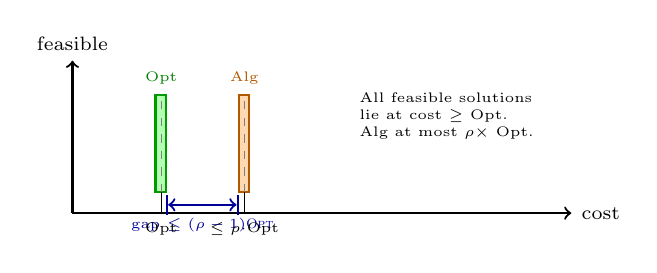
\begin{tikzpicture}[scale=0.88,font=\scriptsize]
\draw[->,thick] (0,0)--(7.2,0) node[right] {cost};
\draw[->,thick] (0,0)--(0,2.2) node[above] {feasible};
\fill[green!30,draw=green!60!black,thick] (1.2,0.3) rectangle (1.35,1.7);
\node[green!50!black,font=\tiny] at (1.28,1.95) {Opt};
\fill[orange!30,draw=orange!70!black,thick] (2.4,0.3) rectangle (2.55,1.7);
\node[orange!70!black,font=\tiny] at (2.48,1.95) {Alg};
\draw[|<->|,thick,blue!60!black] (1.35,0.12)--(2.4,0.12) node[midway,below=1pt,font=\tiny] {gap $\le(\rho-1)\textsc{Opt}$};
\foreach \x/\lab in {1.28/Opt,2.48/$\le\rho\cdot$Opt} \draw (\x,0.3)--(\x,0) node[below,font=\tiny] {\lab};
\node[align=left,font=\tiny] at (5.4,1.4) {All feasible solutions\\ lie at cost $\ge$ Opt.\\ Alg at most $\rho\times$ Opt.};
\draw[dashed,gray] (1.28,0.3)--(1.28,1.7);
\draw[dashed,gray] (2.48,0.3)--(2.48,1.7);
\end{tikzpicture}
\caption{Approximation ratio as a bounded gap above the (unknown) optimum. We never compute Opt, yet we bound Alg relative to it.}
\label{fig:approx-ratio}
\end{figure}

% ============================================================
\section{Vertex Cover: A $2$-Approximation from Maximal Matching}
\label{sec:vertex-cover}

\textsc{Vertex Cover}: given $G=(V,E)$, find smallest $C\subseteq V$ touching every edge. Decision version is $\mathsf{NP}$-complete.

\textbf{Idea before proof:} pick an edge, any cover must take at least one endpoint. So pick \emph{both} endpoints, delete incident edges, repeat. The edges we picked are disjoint (a matching), so any cover needs $\ge$ one vertex per picked edge --- our solution uses exactly $2$ per edge.

\begin{figure}[h]\centering
\begin{tikzpicture}[scale=0.78,font=\scriptsize,every node/.style={circle,draw,fill=blue!12,inner sep=2pt,minimum size=14pt}]
\node (a) at (0,1.2) {$a$}; \node (b) at (1.6,1.2) {$b$}; \node (c) at (3.2,1.2) {$c$};
\node (d) at (0,0) {$d$}; \node (e) at (1.6,0) {$e$}; \node (f) at (3.2,0) {$f$};
\draw[ultra thick,red!70!black] (a)--(b); \draw (b)--(c); \draw (a)--(d); \draw (b)--(e); \draw (c)--(f); \draw (d)--(e);
\node[draw=none,fill=none,font=\tiny,rectangle] at (1.6,-0.85) {Red = picked matching edge; Alg takes both endpoints};
\begin{scope}[on background layer]
\fill[orange!18,rounded corners] (-0.4,-0.4) rectangle (2.0,1.6);
\end{scope}
\node[draw=none,fill=none,font=\tiny,orange!70!black] at (5.0,0.9) {Alg cover: $\{a,b,d,e\}$};
\node[draw=none,fill=none,font=\tiny,green!50!black] at (5.0,0.35) {Opt $\ge2$ (one/edge) $\to2$-approx};
\end{tikzpicture}
\caption{Maximal matching (red) yields a $2$-approximation: any cover needs one endpoint per matching edge; Alg uses two.}
\label{fig:vc-matching}
\end{figure}

\begin{lstlisting}[language=Python]
def vertex_cover_2approx(adj):
    """adj: dict v -> set(neighbors). Returns 2-approx vertex cover."""
    cover = set()
    # maximal matching: greedily pick uncovered edges
    uncovered = {(u,v) for u in adj for v in adj[u] if u < v}
    matching = []
    while uncovered:
        u, v = uncovered.pop()
        matching.append((u, v))
        cover.update([u, v])
        # remove all edges incident to u or v
        uncovered = {(a,b) for (a,b) in uncovered if a not in (u,v) and b not in (u,v)}
    return cover  # |cover| = 2*|matching| <= 2*OPT
\end{lstlisting}

\begin{theorem}[\textsc{Vertex Cover} $2$-approximation]
The matching algorithm returns $C$ with $|C|\le 2\cdot\textsc{Opt}$ in $O(|V|+|E|)$ time.
\end{theorem}
\begin{proof}
Let $M$ be the matching found. Any cover must contain $\ge 1$ endpoint of each $e\in M$, and edges of $M$ are disjoint, so $\textsc{Opt}\ge |M|$. The algorithm outputs $|C|=2|M|\le 2\cdot\textsc{Opt}$. Maximality guarantees every edge touches $M$, so $C$ is a valid cover. Linear scan gives $O(|V|+|E|)$.
\end{proof}

Tight example: a complete bipartite $K_{n,n}$ makes the ratio approach $2$.

% ============================================================
\section{TSP: When Geometry Saves You}
\label{sec:tsp}

\textsc{TSP} (general) has no $O(1)$-approximation unless $\mathsf{P}=\mathsf{NP}$. But \emph{metric} TSP (distances satisfy triangle inequality + symmetry) admits constant factors.

\textbf{MST doubling ($2$-approx):} compute MST $T$ ($c(T)\le\textsc{Opt}$ since removing one edge from Opt tour gives a spanning tree), double its edges to get Eulerian tour, shortcut repeated vertices via triangle inequality --- cost at most $2c(T)\le 2\cdot\textsc{Opt}$.

\textbf{Christofides ($3/2$-approx):} find MST, let $O$ be odd-degree vertices ($|O|$ even), compute minimum perfect matching $M$ on $O$ ($c(M)\le\textsc{Opt}/2$ by shortcutting Opt on $O$), combine $T\cup M$ (Eulerian), shortcut. Total $\le\textsc{Opt}+\textsc{Opt}/2=3\textsc{Opt}/2$.

\begin{lstlisting}[language=Python]
import networkx as nx  # conceptual; any MST impl works
def tsp_mst_double_approx(G):
    """G: complete metric graph with weight 'w'. Returns 2-approx tour cost bound."""
    T = nx.minimum_spanning_tree(G, weight='w')
    mst_cost = sum(d['w'] for _,_,d in T.edges(data=True))
    # Doubling + shortcutting never exceeds 2*mst_cost by triangle inequality
    return 2 * mst_cost  # upper bound; actual shortcut tour <= this
\end{lstlisting}

% ============================================================
\section{Set Cover: Greedy $\ln n$ and Its Limit}
\label{sec:set-cover}

Universe $U$ ($|U|=n$), family $\mathcal{S}=\{S_1,\dots,S_m\}$ with costs, cover all elements. Greedy: repeatedly pick the set minimising cost per newly covered element.

\begin{theorem}[Greedy $\ln n$-approximation]
For unit costs, greedy returns $\le H_n\cdot\textsc{Opt}\le(\ln n+1)\cdot\textsc{Opt}$ where $H_n=1+\tfrac12+\cdots+\tfrac1n$.
\end{theorem}
\begin{proof}[Sketch]
Charge each newly covered element $e$ price $\text{price}(e)=1/|S^*\cap R|$ where $S^*$ is the chosen set and $R$ the remaining uncovered set. Order elements by coverage time $e_1,\dots,e_n$. When $k$ elements remain, some optimal set covers $\ge k/\textsc{Opt}$ of them (pigeonhole over $\textsc{Opt}$ sets), so greedy pays $\le\textsc{Opt}/k$ per element. Summing: $\sum_{k=1}^{n}\textsc{Opt}/k=H_n\cdot\textsc{Opt}$. Tightness follows from set-system constructions achieving $(1-o(1))\ln n$.
\end{proof}

No polynomial algorithm achieves $(1-\varepsilon)\ln n$ unless $\mathsf{P}=\mathsf{NP}$ (Feige).

% ============================================================
\section{LP Rounding: Vertex Cover Revisited}
\label{sec:lp-rounding}

Integer program for \textsc{Vertex Cover}:
\[
\min\sum_{v}x_v \;\text{s.t.}\; x_u+x_v\ge 1\;\forall (u,v)\in E,\; x_v\in\{0,1\}.
\]
Relax to $0\le x_v\le 1$ (LP), solve in polynomial time to get $x^*$, then round: take $C=\{v:x^*_v\ge 1/2\}$.

\begin{theorem}[LP rounding is $2$-approximate]
$C$ is a vertex cover with $|C|\le 2\sum_v x^*_v\le 2\cdot\textsc{Opt}_{\text{IP}}$.
\end{theorem}
\begin{proof}
If $(u,v)\in E$, $x^*_u+x^*_v\ge 1$ forces at least one $\ge 1/2$, so $C$ covers $(u,v)$. Also $|C|=\sum_{v\in C}1\le\sum_{v\in C}2x^*_v\le2\sum_v x^*_v$. Since LP optimum $\le$ IP optimum, the bound follows.
\end{proof}
Randomised rounding ($x_v$ taken with prob.\ $x^*_v$) plus alteration gives similar bounds for \textsc{Set Cover} with factor $O(\log n)$.

\begin{figure}[h]\centering
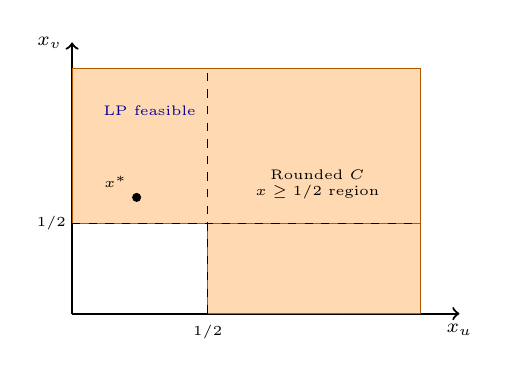
\begin{tikzpicture}[scale=0.82,font=\scriptsize]
\draw[->,thick] (0,0)--(6,0) node[below] {$x_u$}; \draw[->,thick] (0,0)--(0,4.2) node[left] {$x_v$};
\fill[blue!12] (0,2.8)--(4.2,0)--(5.4,0)--(5.4,3.8)--(0,3.8)--cycle;
\draw[thick,red!70!black] (0,2.8)--(4.2,0) node[midway,above,sloped] {$x_u+x_v=1$};
\fill[orange!30,draw=orange!70!black] (2.1,0) rectangle (5.4,3.8);
\fill[orange!30,draw=orange!70!black] (0,1.4) rectangle (5.4,3.8);
\node[font=\tiny,align=center] at (3.8,2.0) {Rounded $C$\\$x\ge 1/2$ region};
\draw[dashed] (2.1,0)--(2.1,3.8); \draw[dashed] (0,1.4)--(5.4,1.4);
\node[font=\tiny] at (2.1,-0.28) {$1/2$}; \node[font=\tiny] at (-0.32,1.4) {$1/2$};
\node[font=\tiny,blue!60!black] at (1.2,3.15) {LP feasible};
\fill (1.0,1.8) circle (2pt) node[above left,font=\tiny] {$x^*$};
\end{tikzpicture}
\caption{LP relaxation of \textsc{Vertex Cover} for one edge. Feasible region above $x_u+x_v\ge1$; rounding at $1/2$ (orange) always hits it and at most doubles cost.}
\label{fig:lp-round}
\end{figure}

% ============================================================
\section{Rounding Beyond Vertex Cover: Set Cover via LP}
\label{sec:lp-setcover}

For \textsc{Set Cover}, the IP is $\min\sum c_i x_i$ s.t.\ $\sum_{i:e\in S_i}x_i\ge1$ for each $e\in U$, $x_i\in\{0,1\}$. Relax to $0\le x_i\le1$, solve, then \emph{randomised rounding}: pick each $S_i$ independently with prob.\ $p_i=\min(1, x^*_i\cdot\ln n)$. Repeat $O(\log n)$ times or use alteration. Each element $e$ is uncovered with prob.\ $\prod_{i:e\in S_i}(1-p_i)\le\exp(-\sum p_i)\le\exp(-\ln n)=1/n$ (since $\sum_{i:e\in S_i}x^*_i\ge1$). Union bound over $n$ elements gives feasibility w.h.p., cost $O(\log n)\cdot\textsc{Opt}_{\text{LP}}$.

\begin{lstlisting}[language=Python]
import random, math
def set_cover_randomized_rounding(sets, costs, x_star, trials=4):
    """Randomised rounding for Set Cover LP. Returns chosen set indices."""
    n_elements = max(max(s) for s in sets) + 1 if sets else 0
    chosen = set()
    for _ in range(trials):
        for i, xi in enumerate(x_star):
            p = min(1.0, xi * math.log(max(2, n_elements)))
            if random.random() < p:
                chosen.add(i)
    return chosen  # w.h.p. covers all elements; cost O(log n)*LP
\end{lstlisting}

% ============================================================
\section{Worked Example: Greedy Set Cover Step-by-Step}
\label{sec:sc-example}

Universe $\{1,2,3,4,5,6\}$, sets $S_1=\{1,2,3\}$, $S_2=\{2,4\}$, $S_3=\{3,4,5\}$, $S_4=\{6\}$, $S_5=\{4,5,6\}$. Greedy picks $S_1$ (covers $3$ new, ratio $1/3$), then $S_5$ (covers $3$ new, ratio $1/3$), total $2$ sets vs.\ Opt $2$ ($S_1+S_5$). Changing $S_1$ to $\{1,2\}$ forces greedy to pick $3$ sets while Opt stays $2$, illustrating the $\ln n$ gap on larger constructions.

% ============================================================
\section{PTAS and Beyond}
\label{sec:ptas}

When does approximation get arbitrarily good? A \emph{PTAS} runs in $n^{f(1/\varepsilon)}$ for ratio $1+\varepsilon$; an \emph{FPTAS} runs in $\text{poly}(n,1/\varepsilon)$; an \emph{EPTAS} in $f(1/\varepsilon)\cdot\text{poly}(n)$. Knapsack has an FPTAS via DP rounding: scale profits by $K=\varepsilon\cdot p_{\max}/n$, run $O(n^3/\varepsilon)$ DP, lose at most $\varepsilon\cdot\textsc{Opt}$. Euclidean TSP has a PTAS (Arora's dissection + DP) but not an FPTAS unless $\mathsf{P}=\mathsf{NP}$. APX-hard problems (e.g., Metric TSP, Max-3SAT) have no PTAS unless $\mathsf{P}=\mathsf{NP}$ --- PCP theorem.

% ============================================================
\section{Chapter Notes}
Vazirani's \emph{Approximation Algorithms} is the classic text; Williamson--Shmoys covers LP/SDP rounding. Christofides (1976) gave $3/2$ for metric TSP, long the best known. Feige (1998) proved $\ln n$ hardness for \textsc{Set Cover}. Recent work improves Euclidean TSP via PTAS (Arora, Mitchell).

% ============================================================
\section{Exercises}
\label{sec:ch01-exercises}
\begin{enumerate}[label=E1.\arabic*, leftmargin=*, itemsep=0.7em]
    \item \textbf{Tight example for VC.} Construct a graph family where the maximal-matching $2$-approximation outputs exactly twice the optimum. Prove both the optimum value and the algorithm's output on your family.
    \item \textbf{Weighted Vertex Cover.} The LP rounding threshold $1/2$ used unit costs. For weights $w_v$, the LP is $\min\sum w_vx_v$. Show the same $1/2$ rounding gives a $2$-approximation for arbitrary weights. Is the factor tight?
    \item \textbf{TSP without triangle inequality.} Prove that if general (non-metric) TSP had a polynomial-time $\rho$-approximation for any $\rho\ge1$, then $\mathsf{P}=\mathsf{NP}$ (hint: reduce Hamiltonian Cycle by setting non-edges to huge cost $\rho n\cdot\max$ edge weight).
    \item \textbf{Set Cover price analysis.} Reproduce the harmonic charging proof for weighted \textsc{Set Cover} where each set $S_i$ has cost $c_i$ and greedy picks minimising $c_i/|S_i\cap R|$. Show the bound $H_{|S_{\max}|}\cdot\textsc{Opt}$.
    \item \textbf{LP integrality gap.} Give a graph where the LP optimum for \textsc{Vertex Cover} is $n/2$ but the IP optimum is $n-1$ (or prove the gap cannot exceed $2$ and exhibit a near-tight instance).
\end{enumerate}
% End of Chapter 1
